\documentclass[conference]{IEEEtran}
\IEEEoverridecommandlockouts
% The preceding line is only needed to identify funding in the first footnote. If that is unneeded, please comment it out.
\usepackage{algorithm}
\usepackage[noend]{algpseudocode}
\usepackage{cite}
\usepackage{amsmath,amssymb,amsfonts}
\usepackage{graphicx}
\usepackage{textcomp}
\usepackage{xcolor}
\def\BibTeX{{\rm B\kern-.05em{\sc i\kern-.025em b}\kern-.08em
    T\kern-.1667em\lower.7ex\hbox{E}\kern-.125emX}}
\begin{document}

\title{Resource Management in Large Language Models\\
}

\author{\IEEEauthorblockN{Xuzhou Zhu}
    \IEEEauthorblockA{522031910324}
    \IEEEauthorblockA{zhuxuzhou@sjtu.edu.cn}
    \and
    \IEEEauthorblockN{Haoyang Pang}
    \IEEEauthorblockA{522031910050}
    \IEEEauthorblockA{1271362703@sjtu.edu.cn}
    \and
    \IEEEauthorblockN{Hanyu Lu}
    \IEEEauthorblockA{522031910043}
    \IEEEauthorblockA{lhy-2785.fanyang@sjtu.edu.cn}
}

\maketitle

\begin{abstract}
    In recent years, there has been a continuous evolution in the scale, performance, and applications of large language models (LLMs),
    progressing from initial models with several million parameters to current models with tens to hundreds of billions of parameters.
    These advancements have led to a continual enhancement in their language understanding and generation capabilities, facilitating their
    widespread adoption across domains such as natural language processing, intelligent customer service, and automated writing.
    Concurrently, trends in transfer learning and open-source sharing have further propelled their applicability and adaptability
    across specific tasks and domains. However, as the parameter count escalates, the demand for computational and storage resources also increases,
    posing a series of challenges and bottlenecks. This survey aims to analyze the existing issues and relevant research efforts in memory management, process scheduling, and computational resource allocation, offering comprehensive insights and valuable perspectives derived from existing literature.
\end{abstract}

\begin{IEEEkeywords}
    LLM, Transformer, Memory Management, Attention Mechanism, Process Scheduling, Distributed Training, Offloading, Inference
\end{IEEEkeywords}

\section{Introduction}
Advancements in LLMs have unlocked novel opportunities across various domains, catalyzing the emergence of a new era of interactive AI applications. Notably, ChatGPT stands out as a pioneering example, facilitating user interaction with AI agents in a conversational manner to address tasks spanning from language translation to software engineering. The remarkable capabilities of ChatGPT have propelled its rapid adoption, positioning it among the fastest-growing applications in history. Numerous organizations have embraced this trend by introducing LLMs and ChatGPT-like applications, exemplified by initiatives such as Microsoft's New Bing, Google's Bard, Meta's LLaMa, Stanford's Alpaca, Databricks' Dolly, and UC Berkeley's Vicuna, among others.However, as LLM models evolve, the increasing volume of data sets and parameters, coupled with elongated context, leads to augmented memory I/O overhead and necessitates optimization of distributed communication structures. These factors collectively impede the development of LLMs. This paper undertakes an analysis of resource management in LLMs from three perspectives: memory management, process scheduling, and allocation of computational resources. Additionally, various strategies and model methodologies for optimizing LLM memory, communication overhead, and computational costs are discussed.

In the memory management section of this survey, we explore two components: the Key-Value (KV) cache and the long-term memory module. The former represents the most prominent source of memory overhead in LLMs, for which we investigate two classical optimization methods: PagedAttention and Tree Attention. The latter incurs additional memory overhead as context grows, and we discuss it through the lens of a Self-Control Memory model. Common memory optimization techniques in large models, such as model compression and distributed storage, while not unique to LLMs, are not elaborated upon in this survey.
In the process scheduling section, we illustrate methods for enhancing model inference speed and reducing computational costs using process scheduling from both the Orca and FastServe models. We also analyze the drawbacks associated with these methods, highlighting novel mechanisms and scheduling strategies for detailed discussion.
In the Computation Resource Management section, this paper examines distributed training and offloading inference from two perspectives. In part A, various parallel optimization schemes existing in distributed training are introduced, including the practical 3D hybrid parallelization widely employed in the industry. Part B discusses current research outcomes in local inference direction through the presentation of two offloading models: FlexGen and PowerInfer.

\section{Memory Management}
During the operation of LLMs, the memory requirements are complex and substantial. In the model training phase, memory is needed for model parameters and gradients, activation values, and optimizer states. During the inference phase, memory is required for model parameters and input data buffers. Recently, as the demand for long-sequence inference has grown, the proportion of memory occupied by the Key-Value cache has increased in order to maintain more contextual information, becoming a focal point for memory optimization.

Therefore, efficient memory allocation is crucial for large language models. Memory not only affects data storage but also plays a crucial role in improving the training and inference speed of the model, reducing memory footprint and resource allocation, and preventing memory leaks.
\subsection{Memory Optimization Based on the Attention Algorithm}
This section primarily focuses on the Attention algorithm, which essentially involves optimizing memory management for the Key-Value (KV) cache.
\subsubsection{PagedAttention}
In long-sequence inference, the KV cache accumulates a significant amount of contextual information regarding keys and values, resulting in substantial memory consumption that dynamically fluctuates, akin to memory allocation challenges encountered in operating systems. Classic OS memory management techniques, like virtual memory and paging, effectively mitigate unnecessary memory usage, enhancing memory utilization. These principles can inform the design of LLMs.

Within the Transformer architecture and its derivatives, the attention mechanism serves as a crucial component for enabling the model to comprehend the relationships among input data. Consequently, integrating paging concepts, like paging the KV cache, should be contemplated within the Attention algorithm. The PagedAttention algorithm \cite{b1}, proposed by Woosuk Kwon and colleagues, offers an illustrative implementation method. Leveraging this insight, vLLM, a service system tailored for LLMs, has been developed.

vLLM is based on the PagedAttention algorithm. The strategy of PagedAttention involves dividing the KV cache of each sequence into multiple blocks, each containing a certain number of tokens' keys and values. For each request to the KV cache, multiple non-contiguous blocks can be allocated. Figure 1 illustrates the storage method of keys and values in the KV cache under the PagedAttention algorithm, while also demonstrating the computation of Query and Key under this storage format.

\begin{figure}[htbp]
    \centerline{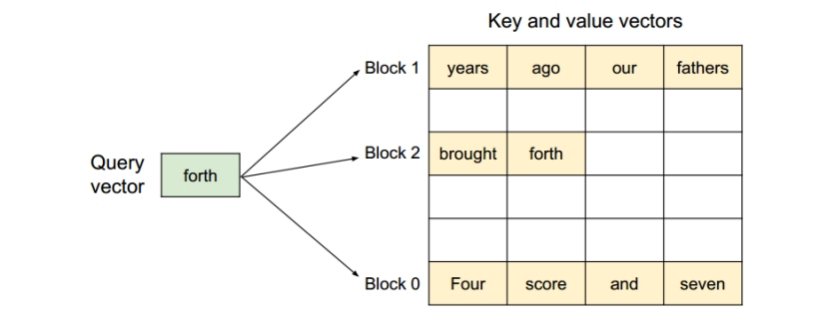
\includegraphics[width=0.5\textwidth]{process figM1.png}}
    \caption{The block storage in the PagedAttention \cite{b1}}
    \label{fig}
\end{figure}

After dividing the KV cache, the original k and v values in the self-attention calculation formula are transformed into k and v vectors corresponding to the blocks in which they are stored. The formula is modified as follows:

\[a_{ij} = \frac{\exp(q_i^{T} \cdot k_j / \sqrt{d})}{\sum_{t=1}^{i} \exp(q_i^{T} \cdot k_t / \sqrt{d})}, \quad o_i = \sum_{j=1}^{i} a_{ij} v_j\]

\[A_{ij} = \frac{\exp(q_i^{T} \cdot K_j / \sqrt{d})}{\sum_{t=1}^{\lceil {i/B} \rceil} \exp(q_i^{T} \cdot K_t1 / \sqrt{d})}, \quad o_i = \sum_{j=1}^{\lceil {i/B} \rceil} V_j A_{ij}^{T}\]

vLLM employs block-level memory management and preemptive request scheduling, both of which are co-designed with PagedAttention. A request’s KV cache is represented as a series of logical KV blocks, filled from left to right as new tokens and their KV cache are generated. Just like the page table in operating system, the KV block manager maintains block tables. Each block table entry records the corresponding physical blocks of a logical block and the number of filled positions. Moreover, the vLLM’s block table has a “filled” record for each block, which represents the number of tokens in that block. If the “filled” record does not equal the maximum capacity that each block can accommodate, then when the key and value of a new token need to be added to the KV cache, the system will first attempt to fill any vacancies in the previous block.

The concept of partitioning the KV cache allows for similar benefits in optimizing KV cache storage space: the space can be non-contiguous, eliminating the external fragmentation caused by contiguous storage. Additionally, the “filled” records also maximize the utilization of each block to a certain extent, thereby reducing internal fragmentation. Moreover, the PagedAttention kernel can process the KV cache in parallel across multiple positions, thereby enhancing hardware utilization and reducing latency.

\subsubsection{Self-Analysis: Combination of vLLM and Distributed Storage}
In vLLM, using a centralized scheduler to coordinate parallel model execution is crucial. This strategy ensures that each model shard can efficiently handle the tasks assigned to it. In this setup, although each GPU processes a part of the entire input, all GPUs still need to access the same set of KV cache data. Therefore, vLLM adopts a centrally managed single KV cache manager to synchronize and share critical data across all computing nodes.

vLLM's design is highly suitable for integration with distributed storage systems, offering the some key advantages: vLLM can implement block allocation and dynamic management of the KV cache. When integrated with distributed storage systems, this architecture can leverage the storage system's dynamic resource allocation capabilities, automatically expanding or contracting storage resources as needed. This not only improves memory utilization but also increases the system's total storage capacity. It also helps to store data close to the computing resources that use this data, thereby reducing data transmission times and enhancing overall processing speed. Moreover, this combination can utilize advanced data backup and fault tolerance mechanisms. In the event of a single node or device failure, the system can automatically recover KV cache data from backups.


\subsubsection{Tree Attention}
In traditional LLMs, keys and values for each output sequence are independently calculated and stored in a KV cache, lacking effective data sharing among sequences with the same prefixes. We can envision tokens as nodes in a tree, facilitating sharing and reuse of computed k and v values during generation.

An example of this idea's application is the SpecInfer engine \cite{b2}, which employs a "Small Speculative Model" (SSM) for tentative speculative inference, depicted in Figure 2. Efficient tree decoding operators enable parallelized inference, and verified paths are output as the model's inference result sequence.

\begin{figure}[htbp]
    \centerline{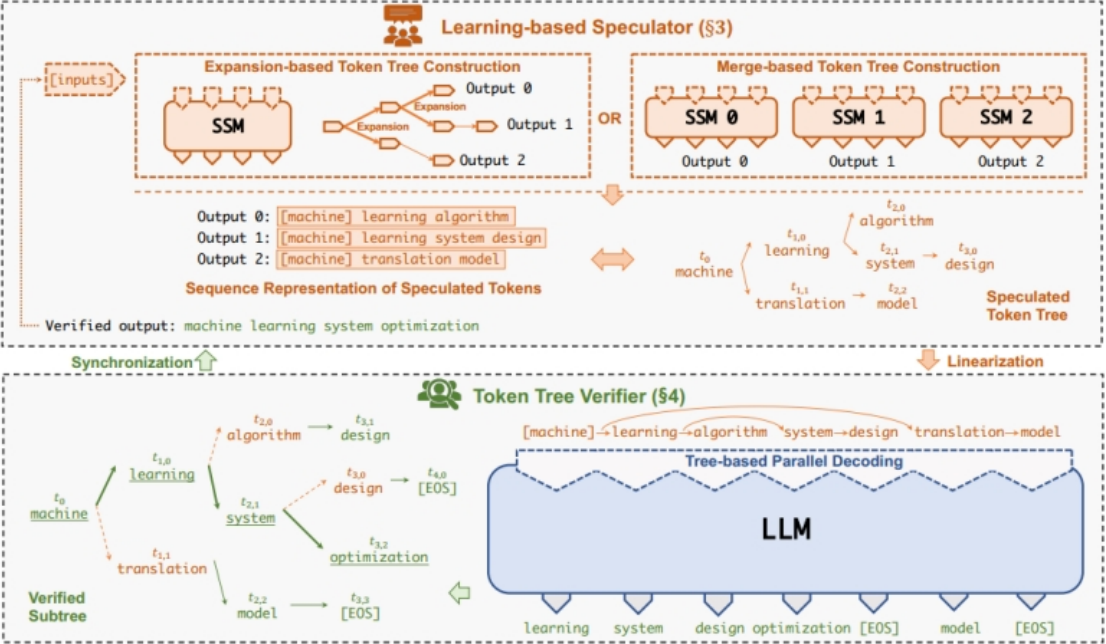
\includegraphics[width=0.5\textwidth]{process figM2.png}}
    \caption{An overview of SpecInfer's tree based speculative inference and verification mechanism \cite{b2}}
    \label{fig}
\end{figure}

Before Tree Attention, SpecInfer breaks down sentences into tokens and utilizes SSM to construct candidate token sequences layer by layer from the root node.

During Tree Attention validation, each candidate token sequence's accuracy must be verified. It calculates probability scores for sequences by appending possible subsequent tokens to the current prefix, achieving parallel verification of multiple tokens. This method allows reuse of k and v values in each layer's computation, reducing memory consumption by avoiding duplicate storage.

Integrating Tree Attention with DFS effectively eliminates redundant KV cache allocations from multiple output sequences sharing the same prefixes, significantly enhancing memory utilization and computational efficiency.

\subsubsection{Summary of Attention Algorithm}
When employing memory optimization strategies based on attention mechanisms, the reduction in memory usage is often not significant, but there is usually a substantial increase in the inference time for LLMs. Essentially, this strategy involves trading time for space. Therefore, when implementing such optimizations, it is crucial to balance computational performance and memory efficiency, making decisions based on specific application requirements.

\subsection{Memory Management in Long-Term Memory and Recall}
In the description above, the term "memory" has two different meanings. The first "memory" refers to the computer's hardware resources, while the second "memory" refers to the recollection of key contextual information that LLMs need to retain when processing lengthy texts.
\subsubsection{Background}
With the development of LLMs, the datasets they rely on have become increasingly vast, and the input they process has become more verbose. When faced with massive amounts of input data, the model's original context-linking capabilities might experience a "forgetting" phenomenon, which is the loss of crucial historical information. To address this issue, memory modules were developed. These modules have become effective tools for handling long-term dependencies, enhancing understanding of context, and improving memory of past information.

There are several main types of memory modules in LLMs. The following will provide a detailed analysis of a specific memory module design called “Self-Controlled Memory System”(SCM) \cite{b3}.

\subsubsection{Implementation and Benefits of SCM}
The SCM system optimizes LLM processing and responsiveness, particularly in memory management. It efficiently stores structured memory items like interaction indices, observations, responses, summaries, and embeddings using caching and vector databases. Memories are categorized into Activation Memory for historical data and Flash Memory for recent interactions, allowing flexible memory utilization.

Memory Activation in the Memory Controller relies on prompts to activate historical memories based on the model's response to current observations. Memories are retrieved and ranked by recency and relevance scores computed from cosine similarity between query and memory embeddings. Only the top k memories (3 to 10) are activated, ensuring pertinent and recent memories are utilized.

Summaries are employed to represent memories if activated memory tokens exceed 2000 and memory length exceeds 800 tokens, reducing data processing volume and maintaining the model within its maximum input length capacity.

\subsubsection{Personal Extended Ideas}
Given the extensive range of memory module designs in LLMs, we have not yet fully explored all these designs. Based on my current knowledge and preliminary understanding of this field, here are some of my thoughts and ideas on memory optimization.

Eviction Policies:

Implementing eviction mechanisms to remove memories that have not been used for an extended period can effectively reduce space consumption. This strategy is analogous to cache eviction algorithms in computer systems and allows for dynamic memory management, ensuring operational efficiency.

Memory Pooling:

Manage memory allocations using memory pools to reduce the overhead associated with frequent memory allocation and deallocation. Memory pools pre-allocate a large block of memory and dynamically allocate or reclaim memory from this block as needed.

Garbage Collection Optimization:

Optimize garbage collection (GC) mechanisms to minimize their impact on system performance. By improving GC algorithms, memory can be managed more effectively without sacrificing response times.

Heterogeneous Storage Strategies:

Employ a combination of different types of storage media (e.g., RAM, SSD, HDD) to store data with varying access frequencies. Frequently accessed "hot" data can be stored on faster media like RAM, while "cold" data can be placed on lower-cost media like HDD.



\section{Process Scheduling}

Inference serving plays a pivotal role in the functionality of interactive AI applications based on LLMs, demanding low job completion times (JCT) to ensure an engaging user experience. However, the substantial size and complexity of LLMs present challenges to inference serving infrastructure, often requiring enterprises to deploy costly clusters equipped with accelerators like GPUs and TPUs. LLM inference possesses unique characteristics that set it apart from other deep neural network (DNN) model inference tasks, such as ResNet \cite{b15}. While DNN inference jobs are typically deterministic and highly predictable \cite{b16}, LLM inference follows a distinct autoregressive pattern. Each iteration of an LLM inference job generates one output token, which is then appended to the input for producing the next output token in the subsequent iteration. The execution time of LLM inference depends on both the input and output lengths, with the latter being unknown beforehand, and that also gives a direction of optimizing.
Therefore, we start from the Transformer model and analyze various process management and scheduling methods available.


\subsection{Iteration-level Scheduling in Orca}
\subsubsection{Problems to Be Solved}


Due to the large scale of models and texts, batch processing is employed to improve efficiency. Traditional LLM serving systems adopt a run-to-completion approach, where a task continues execution until completion without interruption or pause. However, this approach presents issues:
- The input lengths vary, and different requests may require different numbers of iterations, causing some requests to complete prematurely.
Assume there are two requests named x1 and x2. x1 carries a string of “I think this is great”. x2 carries a string of “I love you”. We send the two requests to the transformer.
\begin{figure}[htbp]
    \centerline{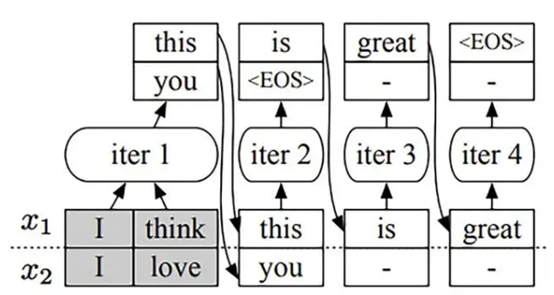
\includegraphics[width=0.5\textwidth]{process fig1.png}}
    \caption{scheduling execution at the request granularity level}
    \label{fig}
\end{figure}
The figure illustrates the scheduling execution at the request granularity level. In this scenario,
although request x2 finishes earlier than request x1, the engine performs computation for both “active” and “inactive” requests throughout all iterations. Such extra computation for inactive requests (x2 at iter 3 and 4) limits the efficiency of batched execution. What makes it even worse is that this behavior prevents an early return of the finished request to the client, imposing a substantial amount of extra latency. This is because the engine only returns the execution results to the serving system when it finishes processing all requests in the batch. Similarly, when a new request arrives in the middle of the current batch’s execution, the newly arrived request must wait until all requests in the current batch have finished. Therefore, this will incur a significant amount of additional computational costs and time overhead. \cite{b10}


\subsubsection{Solution: Iteration-Level Scheduling}


Orca gives a distributed serving system which is utilized for deploying Transformer-based generative models.


Orca addresses this by scheduling each request at a finer granularity (i.e., at each iteration), in FCFS order:

- The iteration-level scheduler repeats the following three steps:

- Selects requests to run next.

- Invokes the engine to execute one iteration for the selected requests.

- Receives execution results for the scheduled iteration.

When the scheduler receives returns after each iteration, it can detect the completion status of requests, promptly returning completed requests to the client. Importantly, new incoming requests only need to wait for one iteration, significantly reducing queuing delays.

\subsubsection{Benefits Transferability of the Iteration-Level Scheduling Strategy}


The transition of the serving system from request granularity to implementing scheduling at each iteration granularity has enhanced overall scheduling flexibility and improved utilization of computational resources.
The scheduler monitors the completion status of requests at each iteration, allowing each completed request to return immediately without waiting for other requests to finish together. The space freed up by returned requests enables new incoming requests to enter, significantly reducing queuing delays.

According to evaluation on a GPT-3 175B model , Orca can significantly outperform NVIDIA FasterTransformer in terms of both latency and throughput: 36.9X throughput improvement at the same level of latency. \cite{b10}


The ability of Large Language Models (LLMs) to perform iteration-level process scheduling and its transferability across different LLM architectures stem from their intrinsic model-agnostic nature. Such scheduling methodologies operate independently of the internal structure of the models, focusing instead on task partitioning and management during iterative computations. Leveraging the parallelism inherent in LLM iterative computations, these scheduling approaches efficiently distribute tasks, irrespective of model specifics, thereby facilitating their migration across diverse LLM frameworks. Furthermore, the reliance on task similarities and the adaptability of scheduling algorithms enable seamless transition and optimization across model boundaries, ensuring their applicability in varied academic contexts.

Thus the iteration-level batch processing (also known as continuous batch processing) method is versatile and can be applied to other models as well, and three examples are shown here:
Utilizing continuous batch processing and model-specific memory optimizations (using vLLM) can increase throughput by up to 23 times.  \cite{b11}
Throughput with continuous batch processing (in Ray Serve and Hugging Face's text generation inference) is 8 times that of naive batch processing. \cite{b12}
By employing optimized models (such as NVIDIA's FasterTransformer), throughput can be increased by 4 times compared to naive batch processing. \cite{b12}

\subsection{FastServe}
\subsubsection{Problems to Be Solved}

Orca implementations used an FCFS strategy without preemptive mechanisms, meaning once a job enters the running state, it must wait until completion. This leads to severe head-of-line blocking issues,which indicates a phenomenon that the delivery of certain packets or tasks is delayed due to the presence of other packets or tasks ahead of them in the queue. Therefore, FastServe, a distributed inference serving system for LLMs, adopts a skip-join Multi-Level Feedback Queue scheduler to implement preemptive scheduling.
\subsubsection{Skip-join Multi-Level Feedback Queue scheduler}


FastServe is based on a preemptive Multi-Level Feedback Queue with a skip-join mechanism (Algorithm 1). Specifically, each job sets a starve timer, and if it waits in the waiting state beyond a threshold, it is promoted to the highest-level queue Q1. Finally, the scheduler selects jobs for execution based on queue priority from highest to lowest.

\begin{algorithm}
    \caption{Skip-Join MLFQ Scheduler  \cite{b10}}
    \begin{algorithmic}
        \State \textbf{Input:} Queues $Q_1, Q_2, ..., Q_k$, jobs $J_{in}$, $J_{pre}$, profiling info $P$
        \State \textbf{Output:} Jobs to be executed $J_{out}$
        \Procedure{SkipjoinMLFQ}{}
        \State \textbf{Initialization:} $J_{out} \leftarrow \emptyset$
        \For{$job \in J_{in}$}
        \State $nextIterTime \leftarrow P.getNextIterationTime(job)$, $p_{job} \leftarrow getHighestPriority(nextIterTime)$
        \State $Q_{p_{job}}.push(job)$
        \EndFor
        \For{$job \in J_{pre}$}
        \State $job.outputNextGeneratedToken()$, $p_{job} \leftarrow job.getCurrentPriority()$
        \If{$job.isFinished()$}
        \State $Q_{p_{job}}.pop(job)$
        \State \textbf{continue}
        \EndIf
        \If{$job.needsDemotion()$}
        \State $nextIterTime' \leftarrow P.getNextIterationTime(job)$
        \State $p_{job}\leftarrow getDemotePrior(p_{job}, nextIterTime')$, $r.demoteTo(Q_{p_{job}})$
        \EndIf
        \EndFor
        \For{$q \in \{Q_2, Q_3, ..., Q_k\}$}
        \For{$job \in q$}
        \If{$job.needsPromotion()$}
        \State $job.promoteTo(Q_1)$, $job.reserveTime()$
        \EndIf
        \EndFor
        \EndFor
        \For{$q \in \{Q_1, Q_2, ..., Q_k\}$}
        \For{$job \in q$}
        \If{$job.isReady()$ and $|J_{out}| < MaxBatchSize$}
        \State $J_{out}.push(job)$
        \EndIf
        \EndFor
        \EndFor
        \EndProcedure
    \end{algorithmic}
\end{algorithm}
In MLFQ eviction, a skip-join mechanism is introduced(figure 4). Before a new job joins the queue, it is evaluated (the reason is explained in next paragraph), and based on the estimated overall execution time using prefill time, it is placed into different priority queues. This aims to prioritize the execution of projects with the least remaining time.

\begin{figure}[htbp]
    \centerline{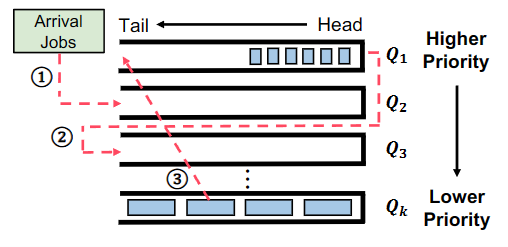
\includegraphics[width=0.5\textwidth]{process fig4.png}}
    \caption{Skip-join MLFQ with starvation prevention}
    \label{fig}
\end{figure}

Specifically, although the number of iterations (i.e., the output length) is not known ahead of time, the execution time of each iteration is predictable. The iteration time is determined by a few key parameters suchas the hardware, the model, and the input length, and thus
can be accurately profiled in advance. Figure below shows the iteration time for GPT-3 2.7B on NVIDIA A100 under different input sequence length. We can see that the first iteration
time (i.e., the execution time to generate the first output token) is longer than those in the decoding phase within a single job. As the input sequence length increases, the first iteration time grows roughly in a linear manner, while the increase of the iteration time in the decoding phase is negligible. This gives the skip-join mechanism information, so the algorithm can decide which queue the new job joins.

\begin{figure}[htbp]
    \centerline{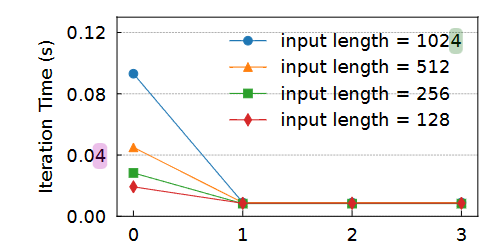
\includegraphics[width=0.5\textwidth]{process fig5.png}}
    \caption{ The execution time of the first four iterations (i.e.first four output tokens) with different input sequence length}
    \label{fig}
\end{figure}

\subsubsection{Benefits and Drawbacks of the Strategy}

The adaption of MLFQ solve the problem of head-of-line blocking
Compared to Orca's non-preemptive scheduling, skip-join MLFQ significantly reduces job completion time and resolves starvation issues, making it superior in terms of time consuming.

However, preemption increases the number of ongoing jobs in the system, and according to measurements, skip-join MLFQ may have a memory overhead 7 times that of FCFS. This preemptive scheduling introduces additional memory overhead, as the KV Cache of each unfinished job must be temporarily stored in memory.


\section{Computation Resource Management}
\subsection{Distributed Training}
With the advancement of LLMs, both model parameters and training datasets are rapidly becoming enormous. To train a mature large-scale model effectively, it is inevitable to employ multiple GPUs for distributed collaborative training to tackle the massive datasets and model parameters that cannot be accommodated on a single card. The crucial issue for large models is how to utilize multi-GPU resources and coordinate information among multiple GPUs. Distributed training nowadays primarily focuses on parallel training through the following three aspects:

\subsubsection{Data parallelism}
Data parallelism involves partitioning massive datasets and maintaining complete models on each GPU. The dataset is divided into 𝑛 parts, and each GPU trains a portion to achieve the training effect. Here, we can discuss two methods of data parallelism in PyTorch classes: DP and DDP.

To achieve effective training across multiple GPUs, it implies that there must be a certain level of information exchange and synchronization among the GPUs. In the torch.nn.DataParallel method, each GPU communicates through a server GPU, responsible for interacting with each GPU, handling information exchange, and summarizing data. Specifically, the server GPU needs to aggregate the forward outputs from each GPU to calculate the loss, compute the gradient of the final layer through the loss, distribute this gradient to each GPU, where each GPU conducts backward propagation independently, and finally aggregate the gradients of all parameters for gradient updates.

Due to the existence of a central GPU, the process is relatively straightforward, with this GPU continuously handling information exchange.
However, the major drawback of this method lies in the central GPU, as its memory and computational capacity become bottlenecks, resulting in low utilization of other GPUs. Hence, this method is not recommended.

With DDP, the most significant structural change is the elimination of the central GPU, thus achieving true distributed effects. To achieve this, we must first introduce a communication method: ring All-Reduce.

Allreduce \cite{b22} : a sum or average of partitioned data which is then shared back to the cluster nodes. In the framework of ring All-Reduce, each GPU holds an equal status, where each GPU only receives data from its left neighbor and sends data to its right neighbor. The entire ring All-Reduce algorithm consists of two steps:
1) scatter-reduce. This step gradually exchanges and merges gradients with each other, resulting in each GPU holding a part of the fully merged gradient. 2) all-gather. This step involves the gradual exchange of incomplete merged gradients, eventually ensuring that all GPUs possess the complete merged gradient.
The entire architecture forms a ring, where information flows cyclically. This enables the successful interaction and merging of all information, hence the term "ring All-Reduce". The theoretical data transmission volume is 2(N−1)×K/N​, where N is the number of GPUs and K is the total data volume per device. The data transferred approaches 2K, while K×N represents the total data volume. Thus, with an increasing number of GPUs, ring All-Reduce can achieve linear scaling.

Returning to DDP, with the premise that ring All-Reduce can achieve linear scaling, we abandon the central GPU and opt for a more evenly balanced distributed system. This is precisely what DDP accomplishes. Therefore, the gradient aggregation function performed by the central GPU in DP is replaced in DDP by allreduce among GPUs. Moreover, since backward does not depend on the aggregated gradient, the allreduce process can be synchronized with backward, further enhancing concurrency and utilization of computational resources.

\subsubsection{Pipeline Parallelism}
Data parallelism only addresses the issue of oversized datasets. In today's LLMs, many model parameters reach several billion, and ChatGPT-4 even surpasses a trillion parameters. In such cases, for distributed training to occur, it is necessary to partition the model.
natural approach is to split the model between different layers, with each GPU holding different layers. Data flows layer by layer between GPUs, sequentially forwarding and backwarding through each layer. This approach solves the problem of storing excessively large models. However, merely doing so doesn't improve computation speed with multiple cards due to communication overhead. In fact, it may prolong training time since only one GPU computes at a time while others remain idle, failing to utilize computational resources effectively.
Pipeline parallelism, inspired by CPU instruction pipelining, introduces GPU computation pipelining in distributed training. The dataset is further divided, with each GPU handling a micro-batch. Once processed, the output is sent to the next GPU, while the current GPU proceeds to handle the next micro-batch. This pipeline design ensures that GPUs are continuously engaged, fully utilizing all computational resources. Consequently, linear acceleration is achievable with an increasing number of GPUs.

\subsubsection{Tensor Parallelism}
As models grow larger, a single GPU may not even accommodate a single layer. In such cases, we consider vertically dividing layers into segments and distributing them across different GPUs. This is where tensor parallelism comes into play.
A tensor, essentially an n-dimensional matrix, is broken down since computations in frameworks like Transformers mainly involve matrix multiplications with linear relationships between parameters. Thus, the overall matrix is divided and matrix multiplications are performed separately, with results subsequently aggregated.
Tensor parallelism entails dividing internal matrices of large models, conducting separate computations, and then aggregating or concatenating outputs using techniques like allreduce. This method is prevalent in LLMs, primarily because modern LLMs are predominantly built upon Transformer architectures, which facilitate tensor parallelism. In contrast, for CNNs, the convolution process is more complex, making it challenging to parallelize through simple matrix partitioning. Hence, this stark difference in parameter quantity between LLMs and CNNs is a significant reason for the former's much larger parameter count.

\subsubsection{ZeRO(Zero Redundancy Optimizer)}
After partitioning and parallelizing datasets and models, as the number of parameters increases, it's evident that certain redundant parts occupy a significant amount of memory. These parts can be further optimized, with one of them being model states.
Model states primarily consist of three components: 1) optimizer states, 2) gradient, 3) model parameter.
ZeRO technology emerges to address the issue of model states consuming a large amount of memory. ZeRO is divided into three levels: ZeRO-1 handles optimizer states, ZeRO-2 handles optimizer states and gradients, and ZeRO-3 handles all model states.
The concept behind ZeRO is relatively straightforward: distribute model states across different GPUs, and during specific steps where complete model states are required, obtain them through allreduce. This increases communication overhead but reduces memory consumption. However, as the number of partitions increases, the corresponding technical intricacies also escalate, and excessive communication may lead to diminishing returns.

\subsubsection{3D Hybrid Parallelism}
By integrating data parallelism, tensor parallelism, pipeline parallelism, and ZeRO technology, with ZeRO-3 inherently partitioning model parameters, overlapping functionalities with tensor parallelism and pipeline parallelism occur. Meanwhile, ZeRO-2 partitions gradients. Combining ZeRO-2 with pipeline parallelism results in significant communication overhead. Hence, when employing 3D parallelism, it is advisable to combine it with ZeRO-1.
Through the coordinated use of multiple parallel strategies, large model parameters can reach the scale of hundreds of billions.

\subsection{Offloading Inference}
For large-scale model training networks, inference is undoubtedly much easier compared to training. However, current commercial inference for large models, such as ChatGPT, is conducted on remote servers, with results transmitted back to users over the network. If it were possible to deploy pre-trained large models locally for inference, it would undoubtedly further expand the application of large models, representing a significant step forward.

When it comes to LLM inference, there are three main directions for reducing computation and storage resources:
1) model compression 2) collaborative inference 3) offloading.
Offloading is one aspect to reduce computation and storage resources for LLM inference. it makes full use of various hardware resources, transferring parameters from GPU memory to system memory or even disk storage.
Let's delve into two models specifically designed for offloading:

\subsubsection{Flexgen}
FlexGen\cite{b20} aims for the utmost throughput, identifying the most suitable offloading strategy within a specified search space. It utilizes methods like model compression and sparsification to execute inference for models with hundreds of billions of parameters on consumer-grade hosts.
FlexGen can be flexibly configured under various hardware resource constraints by aggregating memory and computation from the GPU, CPU, and disk. Through a linear programming optimizer, it searches for the best pattern to store and access the tensors, including weights, activations, and attention key/value (KV) cache. FlexGen further compresses both weights and KV cache to 4 bits with negligible accuracy loss.

One key idea of FlexGen is to play the latency-throughput trade-off. Achieving low latency is inherently challenging for offloading methods, but the I/O efficiency of offloading can be greatly boosted for throughput-oriented scenarios . FlexGen utilizes a block schedule to reuse weight and overlap I/O with computation, as shown in figure \ref{device fig1}(b) below, while other baseline systems use an inefficient row-by-row schedule, as shown in figure \ref{device fig1}(a) below.
\begin{figure}[htbp]
    \centerline{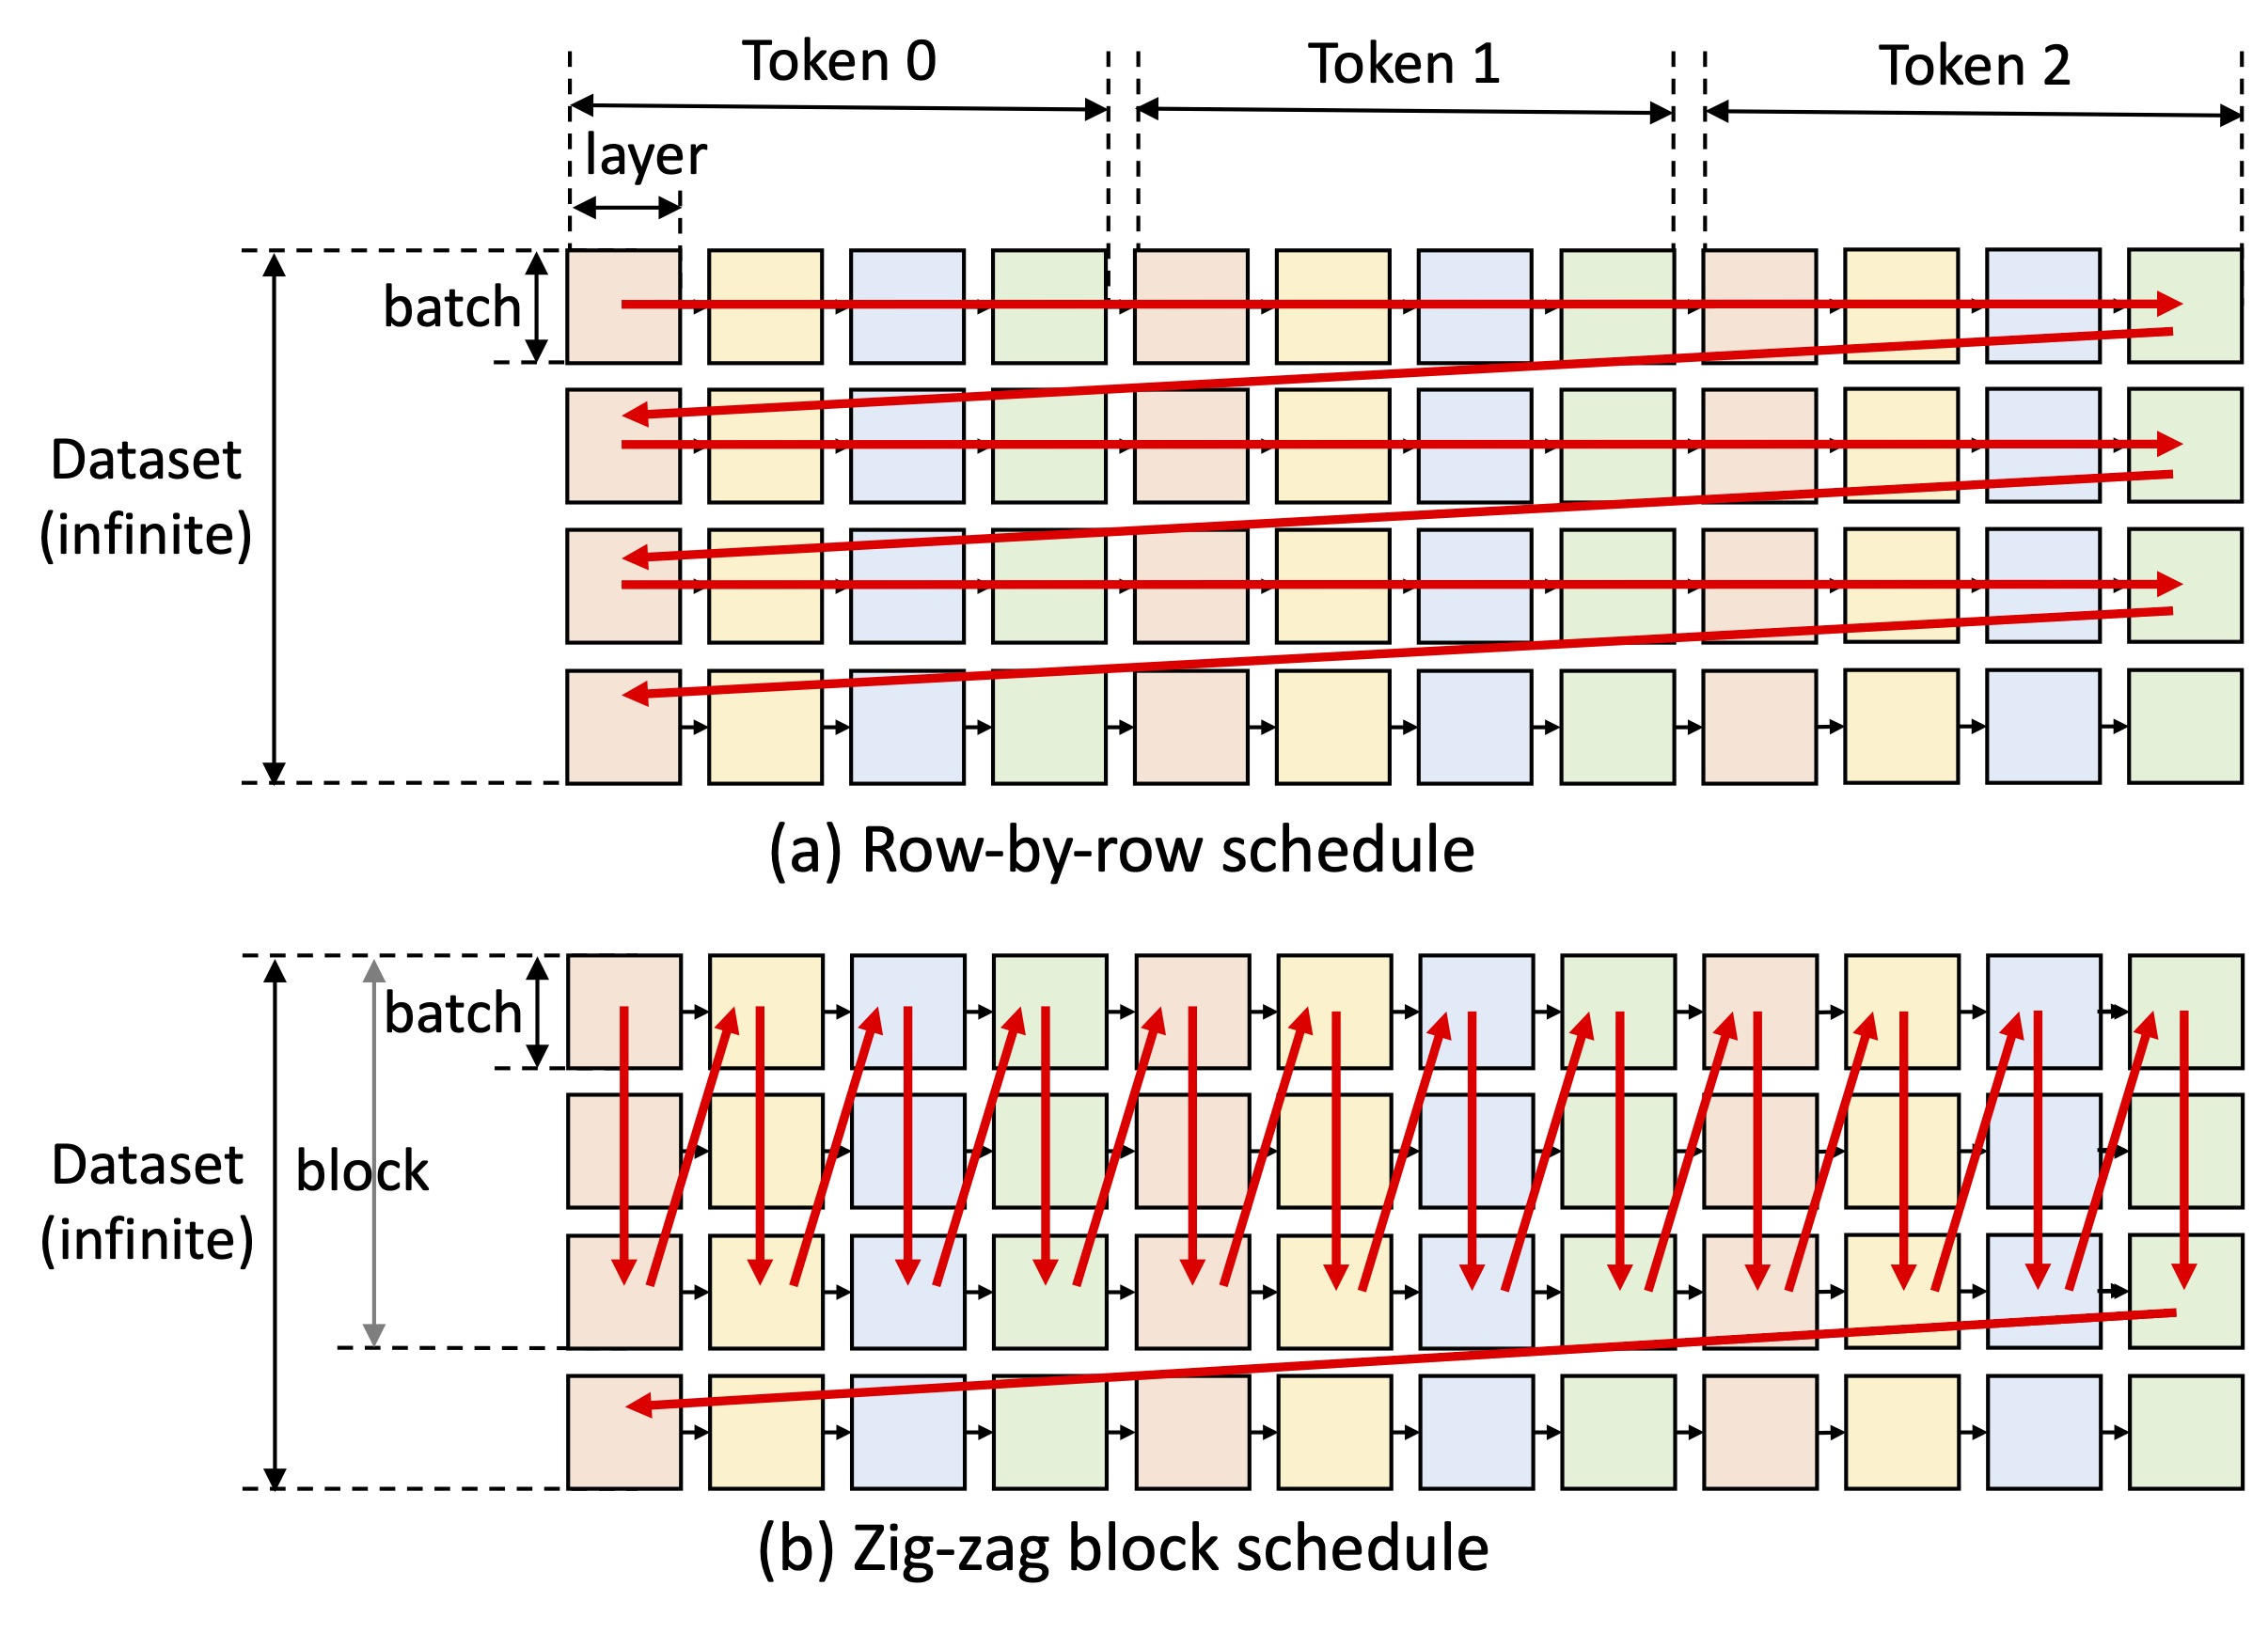
\includegraphics[width=0.5\textwidth]{device fig2.jpg}}
    \caption{two defferent schedules. The red arrows donate the computation order}
    \label{device fig1}
\end{figure}

\subsubsection{PowerInfer}
PowerInfer\cite{b21} partitions neurons into hot and cold neurons based on predictors. During inference, hot neurons are computed on the GPU, while cold neurons are processed on the CPU.
PowerInfer's core idea is essentially sparsity, built upon the fact that only a small portion of neurons are active during the neural network inference process, while the majority remain inactive. Dejavu experiments have verified that over 80\% of neurons and over 95\% of MLP parameters can be excluded from inference\cite{b23}. This implies that a subset of neurons can produce results similar to those of the entire large model. Therefore, placing cold neurons on the CPU for computation would not significantly affect the inference results, as long as the active neurons are computed effectively. Additionally, since cold and hot neurons are pre-determined, the data exchange and communication overhead during inference would be considerably reduced.
figure \ref{device fig2} illustrates the logical structure of PowerInfer.
\begin{figure}[htbp]
    \centerline{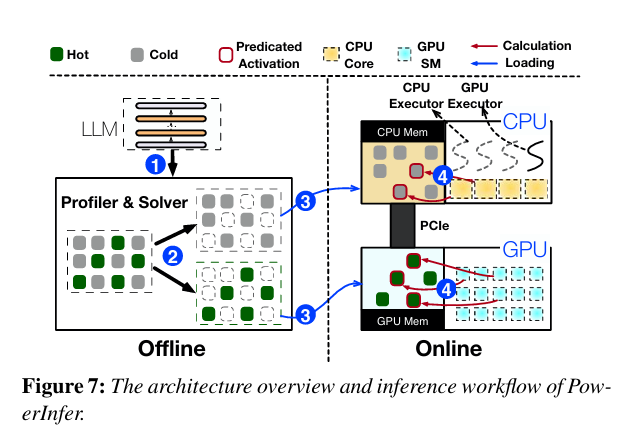
\includegraphics[width=0.5\textwidth]{device fig1.png}}
    \caption{The architecture overview and inference workflow of PowerInfer.}
    \label{device fig2}
\end{figure}
The final implementation of PowerInfer has shown remarkable effectiveness. When compared with llama.cpp across various models such as Opt 66B, Opt 175B, Falcon 40B, and Llama 70B, it has achieved several-fold acceleration for different output lengths and data precisions.

PowerInfer's approach is novel, particularly in its prediction of cold and hot neurons, which offers an innovative perspective. The demonstration results are quite impressive, showcasing significant speed improvements. However, the practicality of this approach still needs improvement. Its model adaptability is somewhat cumbersome, as it is only suitable for models using the ReLU activation function. Models utilizing SILU activation require fine-tuning for a ReLU version. Additionally, this method is lossy, which raises questions about its compatibility with further developments in quantization. Whether PowerInfer can coexist with quantization is also a worthwhile consideration.

\section{Conclusion}
In the resource management of Large Language Models (LLMs), optimization of memory and computational resources constrains each other. Among the various optimization methods for both memory and computational resources mentioned above, the optimization of one often leads to redundancy in the other. In many cases, it is necessary to decide whether to use specific optimization methods based on the specific application scenarios and requirements of the model. We also look forward to more advanced hardware support and design optimization in the future to overcome this dilemma.

\section{Acknowledgment}

\begin{thebibliography}{00}
    \bibitem{b1} Kwon W, Li Z, Zhuang S, et al. Efficient memory management for large language model serving with pagedattention[C]//Proceedings of the 29th Symposium on Operating Systems Principles. 2023: 611-626.
    \bibitem{b2} Miao X, Oliaro G, Zhang Z, et al. SpecInfer: Accelerating Large Language Model Serving with Tree-based Speculative Inference and Verification[C]//Proceedings of the 29th ACM International Conference on Architectural Support for Programming Languages and Operating Systems, Volume 3. 2024: 932-949.
    \bibitem{b3} Wang B, Liang X, Yang J, et al. Enhancing large language model with self-controlled memory framework[J]. arXiv e-prints, 2023: arXiv: 2304.13343.

    \bibitem{b10} Yu G I, Jeong J S, Kim G W, et al. Orca: A distributed serving system for Transformer-Based generative models[C]//16th USENIX Symposium on Operating Systems Design and Implementation (OSDI 22). 2022: 521-538.
    \bibitem{b11} Kwon W, Li Z, Zhuang S, et al. Efficient memory management for large language model serving with pagedattention[C]//Proceedings of the 29th Symposium on Operating Systems Principles. 2023: 611-626.
    \bibitem{b12} Cade Daniel, Chen Shen, Eric Liang, et al.  How continuous batching enables 23x throughput in LLM inference while reducing p50 latency. https://www.anyscale.com/blog/continuous-batching-llm-inference
    \bibitem{b13} NVIDIA docs, last resumed in Feb. 2023 https://docs.nvidia.com/deeplearning/performance/dl-performance-gpu-background/index.html understand-perf
    \bibitem{b14} Wu B, Zhong Y, Zhang Z, et al. Fast distributed inference serving for large language models[J]. arXiv preprint arXiv:2305.05920, 2023.
    \bibitem{b15} He K, Zhang X, Ren S, et al. Deep residual learning for image recognition[C]//Proceedings of the IEEE conference on computer vision and pattern recognition. 2016: 770-778.
    \bibitem{b16} Gujarati A, Karimi R, Alzayat S, et al. Serving DNNs like clockwork: Performance predictability from the bottom up[C]//14th USENIX Symposium on Operating Systems Design and Implementation (OSDI 20). 2020: 443-462.

    \bibitem{b20}Sheng Y, Zheng L, Yuan B, et al. Flexgen: High-throughput generative inference of large language models with a single gpu[C]//International Conference on Machine Learning. PMLR, 2023: 31094-31116.
    \bibitem{b21}Song Y, Mi Z, Xie H, et al. Powerinfer: Fast large language model serving with a consumer-grade gpu[J]. arXiv preprint arXiv:2312.12456, 2023.
    \bibitem{b22}Zhao H, Canny J. Sparse allreduce: Efficient scalable communication for power-law data[J]. arXiv preprint arXiv:1312.3020, 2013.
    \bibitem{b23}Liu Z, Wang J, Dao T, et al. Deja vu: Contextual sparsity for efficient llms at inference time[C]//International Conference on Machine Learning. PMLR, 2023: 22137-22176.
\end{thebibliography}
\vspace{12pt}
\end{document}
